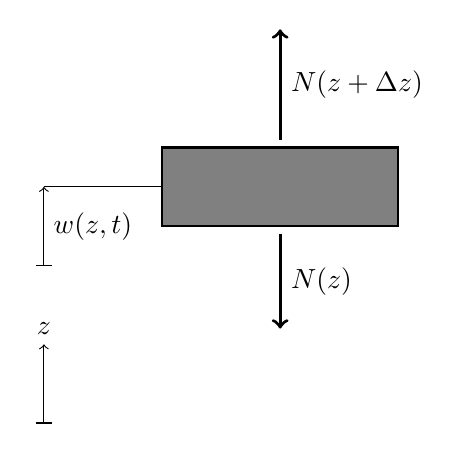
\begin{tikzpicture}
          \draw[thick, fill=gray] (-1.5,-0.5) rectangle (1.5,0.5);
          \draw[->] (-3,-3) -- (-3,-2) node[above] {$z$};
          \draw (-3.1,-3) --(-2.9,-3);
          \draw[->] (-3,-1) -- node[right] {$w(z,t)$} (-3,0);
          \draw (-3.1,-1) --(-2.9,-1);
          \draw (-3,0) -- (-1.5,0);
          \draw[->, very thick] (0, 0.6) -- node[right] {$N(z+\Delta z)$} (0, 2);
          \draw[->, very thick] (0,-0.6) -- node[right] {$N(z)$} (0,-1.8);
\end{tikzpicture}
 
